\documentclass[a4paper, fleqn]{article}

\date{\today}
\author{Hugh Delaney}
\title{5615 CUDA---Assignment 3 \\ Exponential Integral Calculation}

\usepackage[utf8]{inputenc}
\usepackage[T1]{fontenc}
\usepackage{textcomp}
\usepackage{amsmath, amssymb, amsthm}
\usepackage{mathtools, geometry}
\geometry{left=2.5cm,right=2.5cm,top=2.5cm,bottom=2.5cm}
\usepackage{xcolor}
\usepackage{listings}

\DeclarePairedDelimiterX{\inp}[2]{\langle}{\rangle}{#1, #2}

\setlength{\mathindent}{1cm}

% figure support
\usepackage{import}
\usepackage{xifthen}
\pdfminorversion=7
\usepackage{pdfpages}
\usepackage{caption, subcaption}
\usepackage{transparent}
\newcommand{\incfig}[1]{%
        \def\svgwidth{\columnwidth}
        \import{./figures/}{#1.pdf_tex}
}

\definecolor{codegreen}{rgb}{0,0.6,0}
\definecolor{codegray}{rgb}{0.5,0.5,0.5}
\definecolor{codepurple}{rgb}{0.58,0,0.82}
\definecolor{backcolour}{rgb}{0.95,0.95,0.92}

\lstdefinestyle{mystyle}{
    backgroundcolor=\color{backcolour},   
    commentstyle=\color{codegreen},
    keywordstyle=\color{magenta},
    numberstyle=\tiny\color{codegray},
    stringstyle=\color{codepurple},
    basicstyle=\ttfamily\footnotesize,
    breakatwhitespace=false,         
    breaklines=true,                 
    captionpos=b,                    
    keepspaces=true,                 
    numbers=left,                    
    numbersep=5pt,                  
    showspaces=false,                
    showstringspaces=false,
    showtabs=false,                  
    tabsize=2
}

\lstset{style=mystyle}



\pdfsuppresswarningpagegroup=1

\newtheorem{theorem}{Theorem}[section]
\newtheorem{definition}[theorem]{Definition}
\newtheorem{corollary}{Corollary}[theorem]
\newtheorem{proposition}{Proposition}[theorem]
\newtheorem{lemma}[theorem]{Lemma}
\newtheorem{remark}{Lemma}[theorem]

\renewcommand\qedsymbol{$\blacksquare$}

\begin{document}
\maketitle
        \section{CUDA Implementation}%
        \label{sec:cuda_implementation}
        
        Please see \texttt{gpu\_funcs.cu}. \texttt{make prof1} will run the code on 1 GPU, and \texttt{make prof2} will run code on 2 GPUs. 

        Advanced techniques used:
        \begin{itemize}
                \item Constant/Shared memory---constant memory was used in the first implementations, but it was markedly slower than initializing shared memory with hard coded values. The final implementation uses shared memory as a fast alternative to constant memory.
                \item Multiple Cards/Streams---Multiple cards are used if you provide the \texttt{-s} option. This gives a real boost to performance, especially due to using \texttt{cudaMemcpyAsync()}, which allows memory transfer on one card to overlap with computation on the other card. \texttt{make run2} will run the code on two cards and report individual timings for each card. Since streams are understood to be launched simultaneously, we can take the overall run time as the greater of the two individual timings. 
                \item Dynamic Parallelism---In \texttt{single/gpu\_funcs.cu} please see \texttt{GPU\_exponentialIntegralFloat\_4\_launch()} and 
                        \texttt{GPU\_exponentialIntegralFloat\_4\_execute()}  (note that these functions are not also included in \texttt{double/}). Code can be run dynamically by setting \texttt{bool dynamic=true} in the wrapper function \texttt{launch\_on\_one\_card()}. 

                        Approach consists of launching one thread per n value, and precomputing \texttt{psi} (if \texttt{a<=1.0}), before launching enough threads/blocks to compute the \texttt{numberOfSamples} x values from \texttt{a} to \texttt{b} for that given value of \texttt{n}. This approach was markedly slower than normal non-dynamically parallel approach, so is not used in final fast implementation.
        \end{itemize}

        Advanced techniques considered:
        \begin{itemize}
        \item Texture memory---Texture memory was considered so that we could index between a and b with floating point indexes. However this was decided against since the overhead of creating and initializing texture memory outweighed the cost of creating x values in kernel, which requires no cudaMemcpys before the kernel can start.
        \end{itemize}
\section{Performance}%
\label{sec:performance}

\begin{figure}[hbt!]
        \centering
        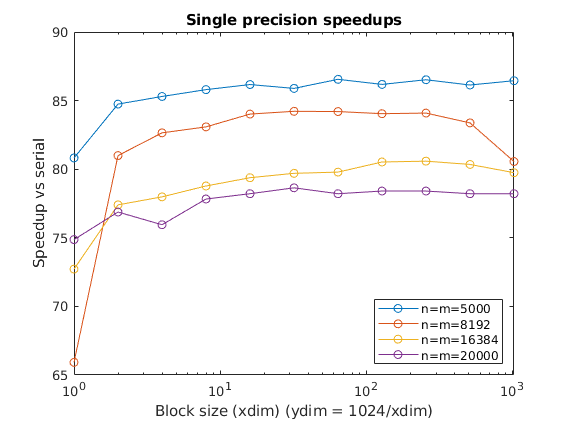
\includegraphics[width=0.8\linewidth]{../single.png}
        \caption{Single Precision Speedups}%
        \label{fig:../single}
\end{figure}
\begin{figure}[hbt!]
        \centering
        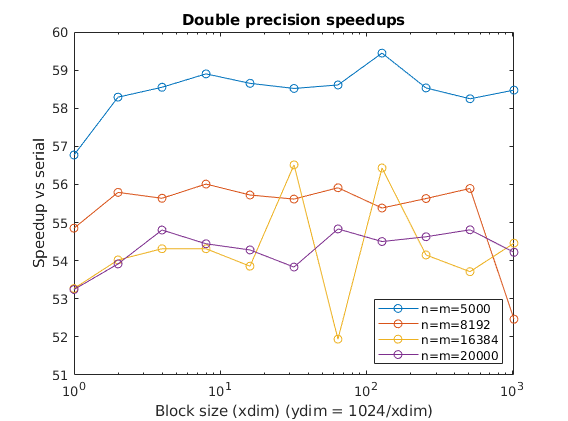
\includegraphics[width=0.8\linewidth]{../double.png}
        \caption{Double Precision Speedups}%
        \label{fig:../double}
\end{figure}
It must first be said that \texttt{blockDim.y = 1024/blockDim.x}, so we are not testing for blocks of different sizes, only different shapes. 

Max error values were around 1E-7 for single precision and around 1E-15 for double precision.

From the figures we can see that block shape does not make a huge difference in the execution speed of our code. Having said that, having a low \texttt{blockDim.x} may give poorer performance than a higher \texttt{blockDim.x}. A consistently good block size seems to be around 16x64, 32x32 or 64x16. 

Notice that speedups actually decrease as n, m grow. This would seem to indicate that the problem is mostly constrained by the bandwidth of the PCI-Express bus, where for bigger problem sizes, data transfer time increases as a proportion of the overall time. I have designed code so as to minimize this data transfer bottleneck, such as by initializing data without the need for any data transfer, as well as by splitting the data transfer over two cards, so that transfers can happen asynchronously using Cuda streams.

There seem to be no algorithmic improvements we can make to our code, since our algorithm is trivially parallel, nor any way to make our on card memory any faster. Dynamic parallelism did not offer any benefits (as far as I can see), as the problem is not simplified by recursion.

In order to increase performance even more, more cards would be needed. However, using a single host node would still cause data bottlenecks to the host, so an MPI/Cuda hybrid solution may work well. In this case we ought to use MPI I/O to write our data to file, instead of causing a bottleneck when transferring data to the master node. 

\end{document}
